\documentclass[conference]{IEEEtran}
\IEEEoverridecommandlockouts
% The preceding line is only needed to identify funding in the first footnote. If that is unneeded, please comment it out.
\usepackage{cite}
\usepackage{amsmath,amssymb,amsfonts}
\usepackage{algorithmic}
\usepackage{graphicx}
\usepackage{textcomp}
\newcommand{\BibTeX}{\textrm{B \kern -.05em \textsc{i \kern -.025em b} \kern -.08em
T \kern -.1667em \lower .7ex \hbox{E} \kern -.125emX}}
\begin{document}

\title{The Efficacy of Chaotic Neural Networks for Asymmetric Encryption of Audio Files}

\author{\IEEEauthorblockN{1\textsuperscript{st} Patrick Pfenning}
\IEEEauthorblockA{\textit{School of Computing and Data Science} \\
\textit{Wentworth Institute of Technology}\\
Boston, MA \\
pfenningp@wit.edu}
}

\maketitle

\begin{abstract}
This document is a model and instructions for \LaTeX.
This and the IEEEtran.cls file define the components of your paper [title, text, heads, etc.]. *CRITICAL: Do Not Use Symbols, Special Characters, Footnotes,
or Math in Paper Title or Abstract.
\end{abstract}

\begin{IEEEkeywords}
component, formatting, style, styling, insert
\end{IEEEkeywords}

\section{Introduction}\label{sec:introduction}

The world we live in has become wildly dependent on fast transfer of information.
Everything from our work and education to our entertainment and social life often requires the internet as a medium.
With this abundance of information, how can one ensure that their personal data remains private to bad actors?
Enter the field encryption, the process of encoding information.
Encryption allows one to take a plaintext message we wish to transmit and transforms it into a ciphertext.
Said ciphertext is illegible to those who do not have a \textit{key}.


Most modern encryption processes create a \textit{psuedo-random} key via a defined algorithm.
These algorithms can be broken into two schemes: \textbf{Symmetric-key Encryption} and \textbf{Public-key Encryption.}
Symmetric-key Encryption algorithms create a single secret-key which both the sender and receiver have.
This key is used to both encrypt and decrypt the message.
The security of this method directly depends on the holders of the key as anyone who has it can read the cipher.
Public-key Encryption algorithms require the message receiver to generate both a public and private key.
The receiver shares the public key with the trusted sender who uses it to encrypt a message.
Said message is sent to the receiver where the private key is used to decrypt it.
Because the private key is the only way to decipher the message, public-keys can be shared with impunity.
Though both methods do nothing to prevent the cipher from being intercepted by a third party, if the algorithm is strong enough, it should be illegible.


Billions of packets of information flow throughout the internet on a daily basis.
The larger the packet, the longer the encryption will.
In this paper we will develop our own algorithm to encrypt several audio files of varying.
The aforementioned algorithm will be developed using what is known as a \textbf{Chaotic Neural Network} (CNN).
This algorithm will be benchmarked for both efficiency and effectiveness against one symmetric-key method, \textbf{Advanced Encryption Standard} (AES), as well as one public-key method, the \textbf{Rivest–Shamir–Adleman} algorithm (RSA).

\section{Literature Review}\label{sec:literature-review}

\subsection{\textbf{Chaos: An Introduction to Dynamical Systems}}\label{subsec:chaos:-an-introduction-to-dynamical-systems}

Alligood~\cite{Alligood} provides an excellent course in the study of such dynamical systems.
She successfully explains chaotic phenomena in nature using Linear Algebra, Differential Equations and Numeric Analysis.
The book defines chaos as a field of study while introducing the idea of chaotic maps.
These maps are recursive in nature, and are highly sensitive to initial conditions.
Each iteration is mapped to a new phase-space for which the rate of separation of points in the sequence is directly related to the system's Lyapunov Exponents.
There is one exponent for each degree of freedom the chosen system has.
The scalar value of the exponent determines how the basis stretch ($LE > 1$) or shrink ($LE < 1$).
Sequences created by such maps, though deterministic, can be unstable.
These unstable sequences are known as chaotic orbits.
This instability is statistically indistinguishable in nature to randomness, making them ideal candidates for providinging repeatable pseudo-random arrays.

\subsection{\textbf{A Review on Applications of Chaotic Maps in Pseudo-Random Number Generators and Encryption}}\label{subsec:a-review-on-applications-of-chaotic-maps-in-pseudo-random-number-generators-and-encryption}

In 2019 Naik and Singh~\cite{Naik2022} gave a detailed review of Chaotic Neural Networks applications for encryption.
The key aspect, as in many of the papers in this section is the creation of a viable generator.
One way chaotic maps are used to generate a sequence of length \textbf{N}, which is equal to the byte-length of the plaintext file.
These values are then converted to binary and one byte are taken from each value, often the first byte after the decimal point.
This sequence is then reshaped to match the dimensions of the file being encrypted.
The resulting matrices are then XORed with the original file masking the data.
If we preform this action a second time, we will revert to the original data.
This is extremely useful for the decryption process.

This paper also goes through another chaotic tool, diffusion, the act of swapping indices.
The Arnold Cat Map (ACM)~\cite{Naik2022} provides an efficient way to diffuse desired file prior to encrypting, but is most often used for image encryption only.
After several iterations of this map on a matrix the original data is unrecognizable.
It should be noted that orbits of ACM are finite, therefore if the map is iterated to the length of the orbit, all diffusion will be undone.

The largest takeaway of this paper is the review of an audio encryption model using sequences from the Henon and Tent maps.
Said sequences are XORed to create a secret key.
This secret key is then XORed with the audio file to encrypt.
Their correlation coefficient between the plain and ciphered files were as low as 0.0014 with entropy was as high as 7.9995.

\subsection{\textbf{Comparison of Cryptography by Chaotic Neural Network and by AES}}\label{subsec:comparison-of-cryptography-by-chaotic-neural-network-and-by-aes}

This 2019 paper by Skovajsová~\cite{Skovajsova2019} gives a step by step explanation of how AES encryption works and compares it to a prebuilt CNN.
Both algorithms were tested on five random images of each of the following sizes: 512b, 1024b, 2048b, 3KB, 30KB and 3MB.
For both ciphering and deciphering, the CNN significantly outperformed the AES model in terms of speed.
The ciphertext created by both models were identical in size to the plaintext file, showing no degradation of information.
It was noted that the CNN used here was a Hopfield network that 1D chaotic maps for its neural weights.
1D maps are much faster for generation, but only require a single initial value.
If this initial condition is found by a bad actor, the algorithm will be broken.
To counteract this, we will be building multiple layer networks of varying dimensionality, each requiring unique sets initial conditions.

\section{Methodology}\label{sec:methodology}

\subsection{Chaotic Functions}\label{subsec:chaotic-functions}

\begin{itemize}
    \item Hénon map
    \item Logistic map
    \item Lorenz system
    \item Tent map
    \item Horseshoe map
    \item \ldots
\end{itemize}

\subsection{Network and Diagram}\label{subsec:network-and-diagram}

Outline inputs and hidden layers here

\begin{figure}[!ht]
    \centering
    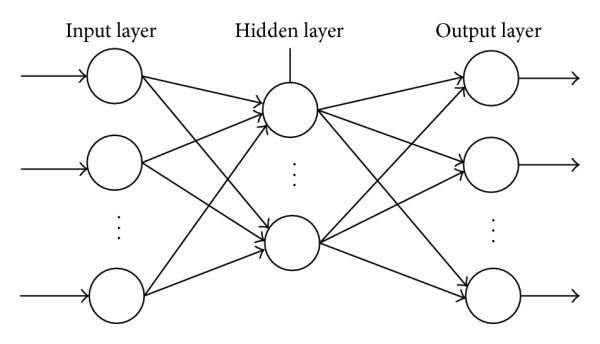
\includegraphics{figures/CNN}
    \caption{Example CNN Architecture}
    \label{fig:CNN}
\end{figure}

\section{Algorithm}\label{sec:algorithm}

\subsection{Key Generation}\label{subsec:key-generation}

\subsection{Diffusion}\label{subsec:diffusion}

\subsection{Encryption}\label{subsec:encryption}

\subsection{Decryption}\label{subsec:decryption}

\subsection{De-Diffusion}\label{subsec:de-diffusion}

\section{Experimentation and Results}\label{sec:experimentation-and-results}

Here we test our algorithm against several existing methods

\subsection{Processing Time and Complexity}\label{subsec:processing-time-and-complexity}

\subsection{Histogram Analysis}\label{subsec:histogram-analysis}

\subsection{Correlation Analysis}\label{subsec:correlation-analysis}

\subsection{Peak Signal to Noise Ratio}\label{subsec:peak-signal-to-noise-ratio}

\subsection{Encryption Quality}\label{subsec:encryption-quality}

\subsection{Vulnerability to Attacks}\label{subsec:vulnerability-to-attacks}

\subsection{Key Sensitivity}\label{subsec:key-sensitivity}

\section{Future Work}\label{sec:future-work}

\section{Conclusion}\label{sec:conclusion}

\section{Acknowledgments}\label{sec:acknowledgments}

\bibliographystyle{ieeetr}
\bibliography{bib/bibliography}

\end{document}
